\documentclass{article}
\usepackage[utf8]{inputenc}
\usepackage{amsmath,amsfonts,amssymb,amsthm,mathtools}
\usepackage{parskip}
\usepackage{booktabs}
\usepackage{tikz}
\usetikzlibrary{calc}

\usepackage[dvipsnames]{xcolor}

\newtheorem{exercise}{Exercise}
\newtheorem{answer}{Answer}

\newcommand{\dd}[2][]{\frac{\partial #1}{\partial #2}}
\newcommand{\dt}[2][]{\frac{d #1}{d #2}}
\newcommand{\dL}{\dt[\L]}
\newcommand{\yh}{\hat{y}}

\newcommand{\bracket}[3]{\left#1 #3 \right#2}
\newcommand{\sqb}{\bracket{[}{]}}
\renewcommand{\b}{\bracket{(}{)}}
\newcommand{\abs}{\bracket{\lvert}{\rvert}}

\newcommand{\x}{\mathbf{x}}
\newcommand{\y}{\mathbf{y}}
\newcommand{\f}{\mathbf{f}}
\newcommand{\h}{\mathbf{h}}
\newcommand{\bv}{\mathbf{b}}
\newcommand{\ov}{\mathbf{o}}
\renewcommand{\a}{\mathbf{a}}
\newcommand{\X}{\mathbf{X}}
\newcommand{\W}{\mathbf{W}}
\newcommand{\I}{\mathbf{I}}
\renewcommand{\P}{\operatorname{P}\b}

\newcommand{\w}{\mathbf{w}}
\newcommand{\wo}{\w^*}

\renewcommand{\L}{\mathcal{L}}
\newcommand{\E}{\operatorname{E}\sqb}
\newcommand{\Var}{\operatorname{Var}\sqb}

\newcommand{\logits}{\ell}
\newcommand{\vlogits}{\boldsymbol{\logits}}
\newcommand{\softmax}{\operatorname{softmax}}
\newcommand{\linear}{\operatorname{linear}}
\newcommand{\relu}{\operatorname{relu}}
\newcommand{\sqerr}{\operatorname{sqerr}}

\newcommand{\func}{\operatorname{func}}
\newcommand{\funcback}{\operatorname{func{.}backward}}
\newcommand{\funcjac}{\operatorname{func{.}jacobian}}
\newcommand{\inputs}{\operatorname{inputs}}
\newcommand{\outputs}{\operatorname{outputs}}

\newcommand{\linearback}{\operatorname{linear{.}backward}}
\newcommand{\reluback}{\operatorname{relu{.}backward}}
\newcommand{\sqerrback}{\operatorname{sqerr{.}backward}}

\newcommand{\linearjac}{\operatorname{linear{.}jacobian}}
\newcommand{\relujac}{\operatorname{relu{.}jacobian}}

\title{SEMT20003, Part 5: Backprop}
\author{Laurence Aitchison}
\date{}

\begin{document}

\maketitle

The key thing about PyTorch that \textit{seems} magical is \verb|backward|, which automatically computes gradients of parameters (or anything else) wrt a loss function.
Ultimately, \verb|backward| applies the backprop algorithm, and the backprop algorithm is just an automatic way of applying the chain rule.  
In this part, we'll:
\begin{enumerate}
  \item Start with a reminder of the multivariable chain rule and total / partial derivatives.
  \item Remind ourselves of the neural network setting. We're going to slightly alter exactly how we write down the neural network, so it'll be easier to talk about backprop later on.
  \item Discuss the high-level strategy for backprop.
  \item Discuss how to backprop is efficiently implemented in PyTorch.
\end{enumerate}

\section{The chain rule, partial and total derivatives}

Unfortunately, the field of deep learning has gotten a bit confused about partial, $\partial$, and total, $d$, derivatives.
I'm going to try to adopt clear and consistent notation.
But I won't always succeede.  
And the field itself is a bit of a mess, so if you look at other resources, you will see other choices of notation.

It is actually simplest to define the partial derivative.  Consider a function of two arguments, $f(x, y)$.
There are two partial derivatives for $f$, one for each argument,
\begin{subequations}
\begin{align}
  \label{eq:ddfx}
  \dd[f]{x} &= \lim_{\Delta x \rightarrow 0} \frac{f(x + \Delta x, y) - f(x, y)}{\Delta x}\\
  \label{eq:ddfy}
  \dd[f]{y} &= \lim_{\Delta y \rightarrow 0} \frac{f(x, y + \Delta y) - f(x, y)}{\Delta y}.
\end{align}
\end{subequations}
Ultimately, the partial derivative takes a \textit{function} (here, $f$) and tells us what happens to the output if you perturb one (and only one) of that function's arguments.

Then we come on to the total derivative.
While you may be more familiar with the total derivative, the total deriative is actually harder to define.
That's because the total derivative describes how changes propagate through a ``compute graph'' (a term from deep learning that turns out to be very useful in our context), not just a single function.
For instance, consider the setting where we have $f(x, y(x))$, i.e.\ $y$ is itself a function of $x$.
The resulting compute graph looks like:
\begin{center}
\begin{tikzpicture}
  \def\xsep{1.8cm}
  \def\de{0.9cm}

  \node (x) at ({0*\xsep}, 0) {$x$};
  \node (y) at ({1*\xsep}, {-\de}) {$y$};
  \node (f) at ({2*\xsep}, 0)      {$f$};

  \draw[->] (x) edge (y);
  \draw[->] (x) edge (f);
  \draw[->] (y) edge (f);
\end{tikzpicture}
\end{center}
The total derivative is what happens in the compute graph, if I add a small perturbation to one of the variables.
For instance, if I add a small perturbation, $dy$ to $y$, then the resulting perturbation to $f$ is,
\begin{align}
  \label{eq:df(dy)}
  df &= \dd[f]{y} dy
\end{align}
Alternatively, if I add a small perturbation, $dx$ to $x$, then the resulting perturbation to $y$ is,
\begin{align}
  \label{eq:dy(dx)}
  dy &= \dd[y]{x} dx
\end{align}
Of course, that same perturbation to $x$ also changes $f$.  The perturbation to $f$ from $dx$ now arises from two sources: directly from $x$ and indirectly through $y$,
\begin{align}
  \label{eq:chain_example}
  df &= \dd[f]{x} dx + \dd[f]{y} dy
  \intertext{substituting the perturbation for $y$ (Eq.~\ref{eq:dy(dx)}),}
  \label{eq:df(dx)}
  df &= \dd[f]{x} dx + \dd[f]{y} \dd[y]{x} dx.
\end{align}
We get the usual total derivatives by ``dividing through'' by $dy$ in Eq.~\eqref{eq:df(dy)} 
\begin{align}
  \dt[f]{y} &= \dd[f]{y}.
\end{align}
i.e.\ the partial and total derivatives for $y$ are the same, because $y$ can only affect $f$ directly, and not through any other ``path''.
And we ``divide through'' by $dx$ in Eq.~\eqref{eq:df(dx)},
\begin{align}
  \dt[f]{x} &= \dd[f]{x} + \dd[f]{y} \dd[y]{x}.
\end{align}
And this is the form for the multivariable chain rule you'll see in most textbook/references.

Thus, the partial and total derivatives for $x$ are different, because they are answering fundamentally different questions.
The partial derivative, $\dd[f]{x}$ is \textit{really} asking how $f$ changes as a function of its first argument, so $x$ is acting as just a ``label'' for the first argument (Eq.~\ref{eq:ddfx}).
In contrast, for the total derivative, we treat $x$ as a component of the compute graph, and ask how a perturbation to $x$ affects $f$ as that perturbation flows through the full graph.

Now, its worth relating my notion of the partial derivative back to something you've heard before, ``the partial deriative is the derivative, holding everything else fixed''.
To see how this alternatie definition differs from my approach, consider a slightly different compute graph, with $f(x(t), y(t))$,
\begin{center}
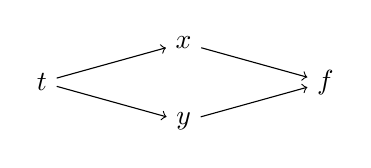
\begin{tikzpicture}
  \def\xsep{1.8cm}
  \def\de{0.5cm}

  \node (t) at (0,         0)      {$t$};
  \node (x) at ({1*\xsep}, { \de}) {$x$};
  \node (y) at ({1*\xsep}, {-\de}) {$y$};
  \node (f) at ({2*\xsep}, 0)      {$f$};

  \draw[->] (t) edge (x);
  \draw[->] (t) edge (y);
  \draw[->] (x) edge (f);
  \draw[->] (y) edge (f);
\end{tikzpicture}
\end{center}
How does the partial derivative work in this context?
The informal definition of the partial derivative usually states ``the partial deriative is the derivative, holding everything else fixed''.
Now, what happens if we try to calculate the partial derivative of $f$ wrt $t$?
This informal definition of the partial derivative would seem to suggest the answer is $0$, as $f$ can't change if we hold $x$ and $y$ fixed,
\begin{align}
  \dd[f]{t} &\stackrel{?}{=} 0.
\end{align}
However, it isn't clear that this makes sense if we look back at our more formal definition of the partial derivative, as ``taking a \textit{function} and telling us what happens to the output if you perturb one (and only one) of that function's arguments''.
Under this more formal definition, it simply does not make sense to ask for the partial derivative of $f$ wrt $t$, as $t$ is not an argument to $f$.  
Instead, $f$ only has two arguments: $x$ and $y$.  
That would suggest,
\begin{align}
  \dd[f]{t} &\stackrel{?}{=} \text{undefined}.
\end{align}
Of course, this is ultimately a matter of definitions, and we are free to choose the definition that is most useful in our specific context.
In deep learning, it's far better to use the more formal definition, as it'll help us to make sense of some of the notational confusion.

In contrast, the total derivative does make sense in this context, as it describes how changes (e.g.\ in $t$) propagate through the full compute graph.
To compute the total derivative, we use the multivariate chain rule,
\begin{align}
  \dt[f]{t} &= \dd[f]{x} \dd[x]{t} + \dd[f]{y} \dd[y]{t}.
\end{align}
This is again the form for the multivariate chain rule you'll find in most textbooks / references.
%Note that the chain rule uses total derivatives for $\dt[x]{t}$ and $\dt[y]{t}$.
%In this simple setting where $x$ and $y$ are univariate functions of $t$, we could equally use partial derivatives.
%But this form for the chain rule continues to work in a more general computational graph where $x$ and $y$ aren't directly functions of $t$, but there's other variables in between.
%\begin{center}
%\begin{tikzpicture}
%  \def\xsep{1.8cm}
%  \def\de{0.5cm}
%
%  \node (t) at (0,         0)      {$t$};
%  \node (a) at ({1*\xsep}, { \de}) {$a$};
%  \node (b) at ({1*\xsep}, {-\de}) {$b$};
%  \node (x) at ({2*\xsep}, { \de}) {$x$};
%  \node (y) at ({2*\xsep}, {-\de}) {$y$};
%  \node (f) at ({3*\xsep}, 0)      {$f$};
%
%  \draw[->] (t) edge (a);
%  \draw[->] (t) edge (b);
%  \draw[->] (a) edge (x);
%  \draw[->] (a) edge (y);
%  \draw[->] (b) edge (x);
%  \draw[->] (b) edge (y);
%  \draw[->] (x) edge (f);
%  \draw[->] (y) edge (f);
%\end{tikzpicture}
%\end{center}
%For instance, in this graph, we introduce new functions, $a, b$ between $t$ and $x, y$.
%In fact, this pre-figures the strategy we're going to use in backprop.  Specifically, remember that Eq.~\eqref{eq:chain_example} continues to make sense.
%But to compute Eq.~\eqref{eq:chain_example} explicitly, we're going to need the total derivatives $\dt[x]{t}$ and $\dt[y]{t}$.
%We can get these total derivatives by applying the chain rule.
%\begin{align}
%  \dt[x]{t} &= \dd[x]{a} \dt[a]{t} + \dd[x]{b} \dt[b]{t},\\
%  \dt[y]{t} &= \dd[y]{a} \dt[a]{t} + \dd[y]{b} \dt[b]{t}.
%\end{align}

[Non-examinable]. 
Hopefully, the previous discussion made some sense, and we'll be using the previously described conventions in the rest of the notes + exam.
However, deep learning folks have made a complete mess of things.
They often write the chain rule entirely in partial deriative form,
\begin{align}
  \dd[f]{t} &= \dd[f]{x} \dd[x]{t} + \dd[f]{y} \dd[y]{t}.
\end{align}
If we directly apply the definitions above, this does not make sense. 
Specifically, $\dd[f]{t}$ is undefined, as $f$ is a function of $x$ and $y$; it is not a function of $t$.
Thus, you could argue that specifying the chain rule in the above form is just wrong (and I'd have alot of sympathy for that argument).
There is an alternative though. 
We could choose to write $f_t$ as a function with one argument, $t$, which gives the same values as $f(x(t), y(t))$,
\begin{align}
  f_t(t) &= f(x(t), y(t)).
\end{align}
Then the argument goes that as $\dd[f]{t}$ is undefined, I must really have meant $\dd[f_t]{t}$.
Indeed it is correct to write,
\begin{align}
  \dd[f_t]{t} &= \dd[f]{x} \dd[x]{t} + \dd[f]{y} \dd[y]{t}.
\end{align}
The problem is that using partial derivatives in this way requires us to constantly implicitly redefine the arguments to our functions. 
It's therefore a really bad idea if we're trying to be precise.
But the fact that deep learning people have got themselves in this mess, but still seem to do useful things probably indicates that it doesn't actually matter too much.

\section{A Scalar Example to Motivate Backprop}
Before diving into the full backprop algorithm, let's look at a simplified example that helps motivate why backprop is useful. Consider a very simple neural network where all variables are scalars rather than vectors. This means:
\begin{itemize}
\item Instead of weight matrices $\W_1$, we have scalar weights $w_1$
\item Instead of bias vectors $\bv_1$, we have scalar biases $b_1$
\item Instead of hidden vectors $\h_1$, we have scalar hidden units $h_1$
\item Instead of activation vectors $\a_1$, we have scalar activations $a_1$
\end{itemize}
Note that the subscripts all indicate layers, not features/datapoints.
The network equations become:
\begin{subequations}
\begin{align}
a_1 &= \linear(x, w_1, b_1) = w_1 x + b_1\\
h_1 &= \relu(a_1)\\
a_2 &= \linear(h_1, w_2, b_2) = w_2 h_1 + b_2\\
h_2 &= \relu(a_2)\\
f &= \linear(h_2, w_3, b_3) = w_3 h_2 + b_3\\
\L &= \sqerr(f, y)
\end{align}
\end{subequations}
where,
\begin{align}
  \sqerr(f, y) &= \tfrac{1}{2} (f - y)^2\\
  \linear(h, w, b) &= w h + b.
\end{align}
The implied compute graph is,
\begin{center}
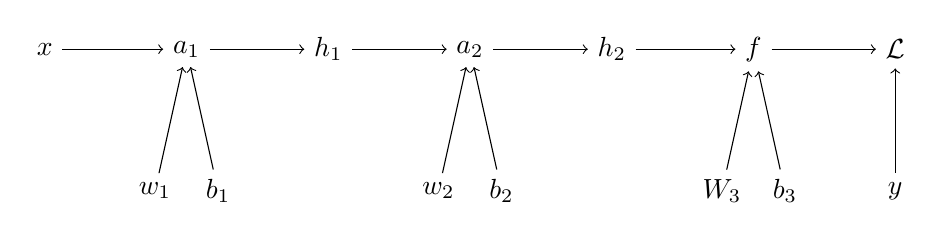
\begin{tikzpicture}
  \def\ysep{1.8cm}
  \def\xsep{1.8cm}
  \def\de{0.4cm}

  \node (x)  at (0, 0) {$x$};
  \node (a1) at ({1*\xsep}, 0) {$a_1$};
  \node (h1) at ({2*\xsep}, 0) {$h_1$};
  \node (a2) at ({3*\xsep}, 0) {$a_2$};
  \node (h2) at ({4*\xsep}, 0) {$h_2$};
  \node (f)  at ({5*\xsep}, 0) {$f$};
  \node (L)  at ({6*\xsep}, 0) {$\L$};

  \node (W1) at ({1*\xsep-\de}, {-\ysep}) {$w_1$};
  \node (b1) at ({1*\xsep+\de}, {-\ysep}) {$b_1$};

  \node (W2) at ({3*\xsep-\de}, {-\ysep}) {$w_2$};
  \node (b2) at ({3*\xsep+\de}, {-\ysep}) {$b_2$};

  \node (W3) at ({5*\xsep-\de}, {-\ysep}) {$W_3$};
  \node (b3) at ({5*\xsep+\de}, {-\ysep}) {$b_3$};

  \node (y)  at ({6*\xsep}, {-\ysep}) {$y$};

  \draw[->] (x) edge (a1);
  \draw[->] (W1) edge (a1);
  \draw[->] (b1) edge (a1);

  \draw[->] (a1) edge (h1);

  \draw[->] (h1) edge (a2);
  \draw[->] (W2) edge (a2);
  \draw[->] (b2) edge (a2);

  \draw[->] (a2) edge (h2);

  \draw[->] (h2) edge (f);
  \draw[->] (W3) edge (f);
  \draw[->] (b3) edge (f);

  \draw[->] (f) edge (L);
  \draw[->] (y) edge (L);
\end{tikzpicture}
\end{center}
Now, our goal is to compute the gradient of the loss wrt all the parameters,
\begin{align}
  &\dL{w_1} &
  &\dL{w_2} & 
  &\dL{w_3} & 
  &\dL{b_1} & 
  &\dL{b_2} & 
  &\dL{b_3}.
\end{align}

Lets do that then!  Applying the chain rule, we get,
\begin{subequations}
\begin{align}
  \dL{w_3} &= \dd[\L]{f} \dd[f]{w_3}\\ %= (f-y) h_2\\
  \dL{b_3} &= \dd[\L]{f} \dd[f]{b_3}\\ %= (f-y)\\
  \dL{w_2} &= \dd[\L]{f} \dd[f]{h_2} \dd[h_2]{a_2} \dd[a_2]{w_2}\\ %= (f-y) w_2 \Theta(a_2) h_1\\
  \dL{b_2} &= \dd[\L]{f} \dd[f]{h_2} \dd[h_2]{a_2} \dd[a_2]{b_2} %= (f-y) w_2 \Theta(a_2)
\end{align}
\end{subequations}
Note that, all the partial derivatives are pretty easy to compute.
For instance,
\begin{align}
  \dd[f]{w_3} &= \dd{w_3}\linear(h_2, w_3, b_3) = \dd{w_3}\sqb{w_3 h_2 + b_3} = h_2.
  \intertext{or,}
  \dd[h_2]{a_2} &= \Theta(a_2)
  \intertext{where,}
  \Theta(a) &= \begin{cases}
     1 & \text{if } a > 0\\
     0 & \text{otherwise}
  \end{cases}
\end{align}
is the gradient of the relu.
etc. While this is all possible in-principle, it is quickly starting to look like alot of painful book-keeping...

Backprop is an algorithm that lets the computer keep track of all the book-keeping for you!
To develop backprop, there are three key insights.

The first key insight is that when we apply the chain rule to compute these derivatives, many of the terms are \textit{shared},
\newcommand{\cola}{\textcolor{red}}
\newcommand{\colb}{\textcolor{blue}}
\newcommand{\colc}{\textcolor{OliveGreen}}
\begin{subequations}
\begin{align}
  \dL{w_3} &= \cola{\dd[\L]{f}} \dd[f]{w_3}\\
  \dL{b_3} &= \cola{\dd[\L]{f}} \dd[f]{b_3}\\
  \dL{w_2} &= \cola{\dd[\L]{f}} \colb{\dd[f]{h_2} \dd[h_2]{a_2}} \dd[a_2]{w_2}\\
  \dL{b_2} &= \cola{\dd[\L]{f}} \colb{\dd[f]{h_2} \dd[h_2]{a_2}} \dd[a_2]{b_2}\\
  \dL{w_1} &= \cola{\dd[\L]{f}} \colb{\dd[f]{h_2} \dd[h_2]{a_2}} \colc{\dd[a_2]{h_1} \dd[h_1]{a_1}} \dd[a_1]{w_1}\\
  \dL{b_1} &= \cola{\dd[\L]{f}} \colb{\dd[f]{h_2} \dd[h_2]{a_2}} \colc{\dd[a_2]{h_1} \dd[h_1]{a_1}} \dd[a_1]{b_1}
\end{align}
\end{subequations}
The second key insight is that these shared terms actually mean something: they're the gradients of the loss wrt the activations:
\begin{subequations}
\begin{align}
  \dL{f} &= \cola{\dd[\L]{f}}\\
  \dL{a_2} &= \cola{\dd[\L]{f}} \colb{\dd[f]{h_2} \dd[h_2]{a_2}}\\
  \dL{a_1} &= \cola{\dd[\L]{f}} \colb{\dd[f]{h_2} \dd[h_2]{a_2}} \colc{\dd[a_2]{h_1} \dd[h_1]{a_1}}.
\end{align}
\end{subequations}
And the third insight is that the gradient of the activations at one layer can be written in terms of the gradients of the activations later in the network,
\begin{subequations}
\begin{align}
  \dL{f} &= \cola{\dd[\L]{f}}\\
  \dL{a_2} &= \dL{f} \colb{\dd[f]{h_2} \dd[h_2]{a_2}}\\
  \dL{a_1} &= \dL{a_2} \colc{\dd[a_2]{h_1} \dd[h_1]{a_1}}.
\end{align}
\end{subequations}
Going even further, and dropping the colours,
\begin{subequations}
\begin{align}
  \dL{f} &= \dd[\L]{f}\\
  \dL{h_2} &= \dL{f} \dd[f]{h_2}\\
  \dL{a_2} &= \dL{h_2} \dd[h_2]{a_2}\\
  \dL{h_1} &= \dL{a_2} \dd[a_2]{h_1}\\
  \dL{a_1} &= \dL{h_1} \dd[h_1]{a_1}.
\end{align}
\end{subequations}
And this is backprop!  We're just going backwards through the network, computing the gradient of the activations at one layer from the gradient at next layer.
We can include parameters too,
\begin{subequations}
\label{eq:scalar:backprop}
\begin{align}
  \dL{f} &= \dd[\L]{f} &&&&\\
  \dL{h_2} &= \dL{f} \dd[f]{h_2} &
  \dL{w_3} &= \dL{f} \dd[f]{w_3} & 
  \dL{b_3} &= \dL{f} \dd[f]{b_3} \\
  \dL{a_2} &= \dL{h_2} \dd[h_2]{a_2} &&&& \\
  \label{eq:scalar:backprop:row}
  \dL{h_1} &= \dL{a_2} \dd[a_2]{h_1} &
  \dL{w_2} &= \dL{a_2} \dd[a_2]{w_2} & 
  \dL{b_2} &= \dL{a_2} \dd[a_2]{b_2} \\
  \dL{a_1} &= \dL{h_1} \dd[h_1]{a_1} &&&&\\
  \textcolor{gray}{\dL{x}}   &\textcolor{gray}{= \dL{a_1} \dd[a_1]{x}} &
  \dL{w_1} &= \dL{a_1} \dd[a_1]{w_1} & 
  \dL{b_1} &= \dL{a_1} \dd[a_1]{b_1}
\end{align}
\end{subequations}
Note that everything in each row can be computed using stuff from the previous row.
The full computation here looks like,
\begin{center}
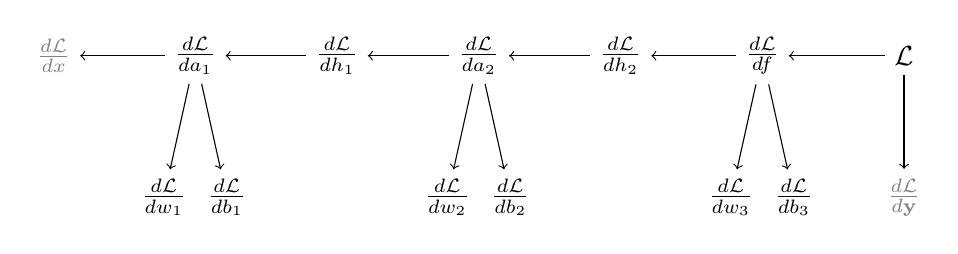
\begin{tikzpicture}
  \def\ysep{1.8cm}
  \def\xsep{1.8cm}
  \def\de{0.4cm}

  \node (x)  at (0, 0) {$\textcolor{gray}{\dL{x}}$};
  \node (a1) at ({1*\xsep}, 0) {$\dL{a_1}$};
  \node (h1) at ({2*\xsep}, 0) {$\dL{h_1}$};
  \node (a2) at ({3*\xsep}, 0) {$\dL{a_2}$};
  \node (h2) at ({4*\xsep}, 0) {$\dL{h_2}$};
  \node (f)  at ({5*\xsep}, 0) {$\dL{f}$};
  \node (L)  at ({6*\xsep}, 0) {$\L$};

  \node[align=right] (W1) at ({1*\xsep-\de}, {-\ysep}) {$\dL{w_1}$};
  \node[align=right] (b1) at ({1*\xsep+\de}, {-\ysep}) {$\dL{b_1}$};

  \node[align=right] (W2) at ({3*\xsep-\de}, {-\ysep}) {$\dL{w_2}$};
  \node[align=right] (b2) at ({3*\xsep+\de}, {-\ysep}) {$\dL{b_2}$};

  \node[align=right] (W3) at ({5*\xsep-\de}, {-\ysep}) {$\dL{w_3}$};
  \node[align=right] (b3) at ({5*\xsep+\de}, {-\ysep}) {$\dL{b_3}$};

  \node (y)  at ({6*\xsep}, {-\ysep}) {$\textcolor{gray}{\dL{\y}}$};

  \draw[<-] (x) edge (a1);
  \draw[<-] (W1) edge (a1);
  \draw[<-] (b1) edge (a1);

  \draw[<-] (a1) edge (h1);

  \draw[<-] (h1) edge (a2);
  \draw[<-] (W2) edge (a2);
  \draw[<-] (b2) edge (a2);

  \draw[<-] (a2) edge (h2);

  \draw[<-] (h2) edge (f);
  \draw[<-] (W3) edge (f);
  \draw[<-] (b3) edge (f);

  \draw[<-] (f) edge (L);
  \draw[<-] (y) edge (L);
\end{tikzpicture}
\end{center}
We have greyed-out $\dL{\x}$ and $\dL{\y}$ because these are gradients wrt data ($\x$ and $\y$), not parameters.
While research papers do sometimes use these papers, that's rare.
In standard settings, data are fixed, not tunable, so we're going to throw away these gradients.

\section{Implementing backprop}

At a mathematical level, that's all there is to backprop.
However, notice that there are still \textit{alot} of equations, and it isn't clear how you'd automated it.
The answer is to notice that I've carefully arranged Eq.~\eqref{eq:scalar:backprop} such that every row computes the gradients of the \textit{inputs} to a particular operation.
For instance, Eq.~\eqref{eq:scalar:backprop:row} computes the gradients of all the inputs to $a_2 = \linear(h_1, w_2, b_2)$.
PyTorch mirrors this arrangement in rows in Eq.~\eqref{eq:scalar:backprop}
%In the previous subsection, we saw that there were two ways to compute the chain rule: Eq.~\eqref{eq:relu:chain} and Eq.~\eqref{eq:relu:back}.
%The first (Eq.~\ref{eq:relu:chain}) explicitly summed over the Jacobian.
%The key insight in the second equation (Eq.~\ref{eq:relu:back}) was that we didn't need the Jacobian explicitly.
%Instead, we just need an expression to compute $\dL{\a}$ from $\dL{\h}$.
%And such an expression can often be much simpler and more efficient than working with Jacobians explicitly.
%This is the key idea behind how backprop is implemented in practice.
Specifically, PyTorch implements ``forward'' for each operation (e.g.\ $\linear$ or $\relu$),
\begin{align}
  \outputs &= \func\b{\inputs}.
\end{align}
PyTorch also gives us a way to apply the chain rule, to compute the gradient of all the inputs, as a function of the gradient of all of the outputs.
\begin{align}
\label{eq:general_forward_backward}
  \dL{\inputs} &= \funcback\b{\dL{\outputs}; \inputs}
\end{align}
This function takes the original inputs, along with the gradient of the objective wrt the output, $\dL{\outputs}$, and returns the gradient of the objective wrt the inputs, $\dL{\inputs}$.

Concretely, for the ReLU:
\begin{subequations}
\begin{align}
  h &= \relu\b{a} \\ 
  \dL{a} &= \reluback\b{\dL{h}; a}
\end{align}
\end{subequations}
And for the linear function,
\begin{subequations}
\begin{align}
  a &= \linear\b{h, w, b} \\ 
  \b{\dL{h}, \dL{w}, \dL{b}} &= \linearback\b{\dL{a}; h, w, b}
\end{align}
\end{subequations}
For the actual value of these derivatives, see the exercises.
Finally, for the sum-square error.
\begin{subequations}
\begin{align}
  \L &= \sqerr\b{f, y} \\ 
  \b{\dL{f}, \dL{y}} &= \sqerrback\b{\dL{\L}=1; f, y}
\end{align}
\end{subequations}
Note that something a little weird happens for the sum-squared error.
Specifically, its output is the loss!
Therefore, $\dL{\outputs}$ becomes $\dL{\L}$.  And of course, $\dL{\L}=1$.

Now, $\funcback$ gives us the gradients of the objective wrt the inputs of the function. 
The inputs to one operation are either:
\begin{itemize}
  \item Parameters, in which case, $\dL{\inputs}$ are the gradients we want (e.g. $\dL{w_3}$).
  \item The output from operation. In that case, $\dL{\inputs}$ from this operation are $\dL{\outputs}$ from the previous operation, so we can pass the gradients backwards.
  \item Data (i.e.\ $\x$ or $\y$), in which case we don't use the gradients.
\end{itemize}
Overall, the full backward pass looks like,
\begin{subequations}
\label{eq:backward}
\begin{align}
  \b{\dL{f}, \textcolor{gray}{\dL{y}}} &= \sqerrback\b{\dL{\L}=1; f, y}\\
  \b{\dL{h_2}, \dL{w_3}, \dL{b_3}} &= \linearback\b{\dL{f}; h_2, w_3, b_3}\\
  \dL{a_2} &= \reluback\b{\dL{h_2}; a_2}\\
  \b{\dL{h_1}, \dL{w_2}, \dL{b_2}} &= \linearback\b{\dL{a_2}; h_1, w_2, b_2}\\
  \dL{a_1} &= \reluback\b{\dL{h_2}; a_2}\\
  \b{\textcolor{gray}{\dL{x}}, \dL{w_2}, \dL{b_2}} &= \linearback\b{\dL{a_1}; x, w_1, b_1}
\end{align}
\end{subequations}
Note that the gradients required as input at each step are computed in the previous step!
%Concretely, we for the ReLU:
%\begin{subequations}
%\begin{align}
%  \h &= \relu\b{\a} \\ 
%  \dL{\a} &= \reluback\b{\dL{\h}; \a}
%\end{align}
%\end{subequations}
%And for the linear function,
%\begin{subequations}
%\begin{align}
%  \a &= \linear\b{\h, \W, \bv} \\ 
%  \b{\dL{\h}, \dL{\W}, \dL{\bv}} &= \linearback\b{\dL{\a}; \h, \W, \bv}
%\end{align}
%\end{subequations}
%For the actual value of these derivatives, see the exercises.
%Finally, for the sum-square error.
%\begin{subequations}
%\begin{align}
%  \L &= \sqerr\b{\f, \y} \\ 
%  \b{\dL{\f}, \dL{\y}} &= \sqerrback\b{\dL{\L}=1; \f, \y}
%\end{align}
%\end{subequations}
%Note that something a little weird happens for the sum-squared error.
%Specifically, its output is the loss!
%Therefore, $\dL{\outputs}$ becomes $\dL{\L}$.  And of course, $\dL{\L}=1$.
%
%Now, $\funcback$ gives us the gradients of the objective wrt the inputs of the function. 
%The inputs to one operation are either:
%\begin{itemize}
%  \item Parameters, in which case, $\dL{\inputs}$ are the gradients we want (e.g. 
%  \item The output from operation. In that case, $\dL{\inputs}$ from this operation are $\dL{\outputs}$ from the previous operation, so we can pass the gradients backwards.
%  \item Data (i.e.\ $\x$ or $\y$), in which case we don't use the gradients.
%\end{itemize}
%Overall, the full backward pass looks like,
%\begin{subequations}
%\label{eq:backward}
%\begin{align}
%  \b{\dL{\f}, \textcolor{gray}{\dL{\y}}} &= \sqerrback\b{\dL{\L}=1; \f, \y}\\
%  \b{\dL{\h_2}, \dL{\W_3}, \dL{\bv_3}} &= \linearback\b{\dL{\f}; \h_2, \W_3, \bv_3}\\
%  \dL{\a_2} &= \reluback\b{\dL{\h_2}; \a_2}\\
%  \b{\dL{\h_1}, \dL{\W_2}, \dL{\bv_2}} &= \linearback\b{\dL{\a_2}; \h_1, \W_2, \bv_2}\\
%  \dL{\a_1} &= \reluback\b{\dL{\h_2}; \a_2}\\
%  \b{\textcolor{gray}{\dL{\x}}, \dL{\W_2}, \dL{\bv_2}} &= \linearback\b{\dL{\a_1}; \x, \W_1, \bv_1}
%\end{align}
%\end{subequations}
%Note that the gradients required as input at each step are computed in the previous step!

Overall, the backprop algorithm is:
\begin{enumerate}
  \item Run the forward pass (Eq.~\ref{eq:forward}), recording the order of and outputs from all operations.
  \item Run the backward pass (Eq.~\ref{eq:backward}) to compute all the gradients, by working backwards through the operations recorded in the forward pass.
\end{enumerate}



\section{From a scalar to a full neural network}

The full network is,
\begin{subequations}
\label{eq:forward}
\begin{align}
  \a_1 &= \linear\b{\x, \W_1, \bv_1}\\
  \h_1 &= \relu\b{\a_1}\\
  \a_2 &= \linear\b{\h_1, \W_2, \bv_2}\\
  \h_2 &= \relu\b{\a_2}\\
  \f &= \linear\b{\h_2, \W_3, \bv_3}\\
  \label{eq:L}
  \L &= \sqerr\b{\f, \y}.
\end{align}
\end{subequations}
where,
\begin{subequations}
\begin{align}
  \label{eq:linear}
  \linear\b{\h, \W, \bv} = \h \W + \bv,\\
  \label{eq:sqerr}
  \sqerr\b{\f, \y} = \tfrac{1}{2} \sum_i (f_i - y_i)^2.
\end{align}
\end{subequations}
The implied compute graph is,
\begin{center}
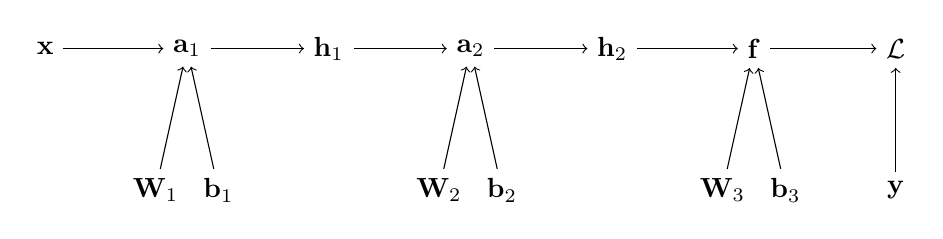
\begin{tikzpicture}
  \def\ysep{1.8cm}
  \def\xsep{1.8cm}
  \def\de{0.4cm}

  \node (x)  at (0, 0) {$\x$};
  \node (a1) at ({1*\xsep}, 0) {$\a_1$};
  \node (h1) at ({2*\xsep}, 0) {$\h_1$};
  \node (a2) at ({3*\xsep}, 0) {$\a_2$};
  \node (h2) at ({4*\xsep}, 0) {$\h_2$};
  \node (f)  at ({5*\xsep}, 0) {$\f$};
  \node (L)  at ({6*\xsep}, 0) {$\L$};

  \node (W1) at ({1*\xsep-\de}, {-\ysep}) {$\W_1$};
  \node (b1) at ({1*\xsep+\de}, {-\ysep}) {$\bv_1$};

  \node (W2) at ({3*\xsep-\de}, {-\ysep}) {$\W_2$};
  \node (b2) at ({3*\xsep+\de}, {-\ysep}) {$\bv_2$};

  \node (W3) at ({5*\xsep-\de}, {-\ysep}) {$\W_3$};
  \node (b3) at ({5*\xsep+\de}, {-\ysep}) {$\bv_3$};

  \node (y)  at ({6*\xsep}, {-\ysep}) {$\y$};

  \draw[->] (x) edge (a1);
  \draw[->] (W1) edge (a1);
  \draw[->] (b1) edge (a1);

  \draw[->] (a1) edge (h1);

  \draw[->] (h1) edge (a2);
  \draw[->] (W2) edge (a2);
  \draw[->] (b2) edge (a2);

  \draw[->] (a2) edge (h2);

  \draw[->] (h2) edge (f);
  \draw[->] (W3) edge (f);
  \draw[->] (b3) edge (f);

  \draw[->] (f) edge (L);
  \draw[->] (y) edge (L);
\end{tikzpicture}
\end{center}
Now, our goal is to compute the gradient of the loss wrt all the parameters,
\begin{align}
  &\dL{\W_1} &
  &\dL{\W_2} & 
  &\dL{\W_3} & 
  &\dL{\bv_1} & 
  &\dL{\bv_2} & 
  &\dL{\bv_3}.
\end{align}
The backward pass again looks like,
\begin{center}
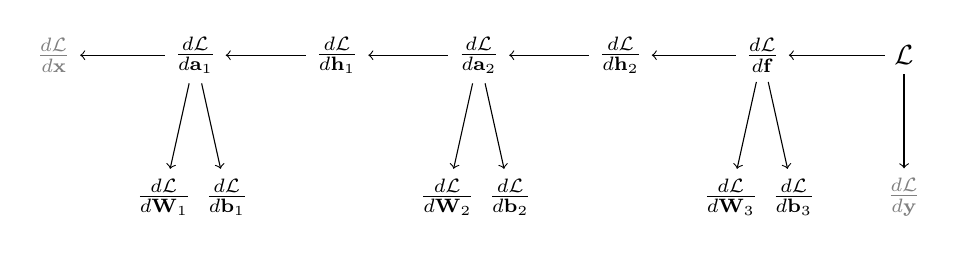
\begin{tikzpicture}
  \def\ysep{1.8cm}
  \def\xsep{1.8cm}
  \def\de{0.4cm}

  \node (x)  at (0, 0) {$\textcolor{gray}{\dL{\x}}$};
  \node (a1) at ({1*\xsep}, 0) {$\dL{\a_1}$};
  \node (h1) at ({2*\xsep}, 0) {$\dL{\h_1}$};
  \node (a2) at ({3*\xsep}, 0) {$\dL{\a_2}$};
  \node (h2) at ({4*\xsep}, 0) {$\dL{\h_2}$};
  \node (f)  at ({5*\xsep}, 0) {$\dL{\f}$};
  \node (L)  at ({6*\xsep}, 0) {$\L$};

  \node[align=right] (W1) at ({1*\xsep-\de}, {-\ysep}) {$\dL{\W_1}$};
  \node[align=right] (b1) at ({1*\xsep+\de}, {-\ysep}) {$\dL{\bv_1}$};

  \node[align=right] (W2) at ({3*\xsep-\de}, {-\ysep}) {$\dL{\W_2}$};
  \node[align=right] (b2) at ({3*\xsep+\de}, {-\ysep}) {$\dL{\bv_2}$};

  \node[align=right] (W3) at ({5*\xsep-\de}, {-\ysep}) {$\dL{\W_3}$};
  \node[align=right] (b3) at ({5*\xsep+\de}, {-\ysep}) {$\dL{\bv_3}$};

  \node (y)  at ({6*\xsep}, {-\ysep}) {$\textcolor{gray}{\dL{\y}}$};

  \draw[<-] (x) edge (a1);
  \draw[<-] (W1) edge (a1);
  \draw[<-] (b1) edge (a1);

  \draw[<-] (a1) edge (h1);

  \draw[<-] (h1) edge (a2);
  \draw[<-] (W2) edge (a2);
  \draw[<-] (b2) edge (a2);

  \draw[<-] (a2) edge (h2);

  \draw[<-] (h2) edge (f);
  \draw[<-] (W3) edge (f);
  \draw[<-] (b3) edge (f);

  \draw[<-] (f) edge (L);
  \draw[<-] (y) edge (L);
\end{tikzpicture}
\end{center}
We have greyed-out $\dL{\x}$ and $\dL{\y}$ because these are gradients wrt data ($\x$ and $\y$), not parameters.
While research papers do sometimes use these papers, that's rare.
In standard settings, data are fixed, not tunable, so we're going to throw away these gradients.

That's great, but how do we actually compute these gradients?
Using the multivariate chain rule.
Specifically, taking Eq.~\eqref{eq:scalar:backprop}, and swapping out all the scalars for vectors, 
%
%By applying the chain rule \textit{alot}.
%We start with $\dL{f_m}$, which can be obtained directly by differentiating Eq.~\eqref{eq:L} using the definition of the squared error function in Eq.~\eqref{eq:sqerr}.
%Then we use the chain rule to compute total derivatives for variables and parameters that appear progressively earlier in the compute graph, 
(I'm not including all the equations here, because it gets quite repetitive),
\begin{subequations}
\label{eq:back_chain}
\begin{align}
  \dL{f_m} &= \dd[\L]{f_m}\\
  %\label{eq:back_chain:1}
  \nonumber
  \dL{h_{2;i}} &= \sum_k \dd[f_k]{h_{3; i}} \dL{f_k}&
  \dL{W_{3;ij}} &= \sum_k \dd[f_k]{W_{3; ij}} \dL{f_k}&
  \dL{b_{3;i}} &= \sum_k \dd[f_k]{b_{3; i}} \dL{f_k}\\
  \dL{a_{2;i}} &= \sum_k \dd[h_{2;k}]{a_{2;i}} \dL{h_{2; k}}\\
  %\dL{h_{3; l}} &= \sum_m \dd[a_{2_m}]{h_{2;l}} \dL{a_{2;m}}\\
  %\dL{h_{2; l}} &= \sum_m \dd[f_m]{h_{2;l}} \dL{f_m}\\
  %%\label{eq:back_chain:2}
  %\nonumber
  %\dL{b_{2;i}} &= \sum_{k} \dd[a_{2; k}]{b_{2; i}} \dL{a_{2; k}}&
  %%\label{eq:back_chain:4}
  %\dL{W_{2;ij}} &= \sum_{k} \dd[a_{2; k}]{W_{2; ij}} \dL{a_{2; k}}\\
  %\dL{h_{2; l}} &= \sum_m \dd[a_{2_m}]{h_{2;l}} \dL{a_{2;m}}\\
  \dots &\phantom{=} \dots
\end{align}
\end{subequations}
Then, we can implement these full Jacobians in code, using,
\begin{subequations}
%\label{eq:backward}
\begin{align}
  \b{\dL{\f}, \textcolor{gray}{\dL{\y}}} &= \sqerrback\b{\dL{\L}=1; \f, \y}\\
  \b{\dL{\h_2}, \dL{\W_3}, \dL{\bv_3}} &= \linearback\b{\dL{\f}; \h_2, \W_3, \bv_3}\\
  \dL{\a_2} &= \reluback\b{\dL{\h_2}; \a_2}\\
  \b{\dL{\h_1}, \dL{\W_2}, \dL{\bv_2}} &= \linearback\b{\dL{\a_2}; \h_1, \W_2, \bv_2}\\
  \dL{\a_1} &= \reluback\b{\dL{\h_2}; \a_2}\\
  \b{\textcolor{gray}{\dL{\x}}, \dL{\W_2}, \dL{\bv_2}} &= \linearback\b{\dL{\a_1}; \x, \W_1, \bv_1}
\end{align}
\end{subequations}
Note that you'll derive these functions in the exercises!

\subsection{Alternative (bad) approach using explicit Jacobians}

To understand just how clever backprop is, its worth going back and trying some alternative approaches.
Specifically, the most obvious approach to implementing backprop is to directly use Eq.~\eqref{eq:back_chain}.
And to do that, we could implement $\funcjac$, which computes the Jacobians, alongside the usual ``forward'' computation,
\begin{subequations}
\label{eq:general_jacobian}
\begin{align}
  \outputs &= \func\b{\inputs}\\
  \dd[\outputs]{\inputs} &= \funcjac\b{\inputs}.
\end{align}
\end{subequations}
Concretely, for the $\relu$ function,
\begin{subequations}
\begin{align}
  \h &= \relu\b{\a} \\ 
  \dd[\h]{\a} &= \relujac\b{\a}
\end{align}
\end{subequations}
Note that $\dd[\h]{\a}$ is just $\dd[h_i]{a_j}$ interpreted as a matrix (like $\mathbf{A}$ vs $A_{ij}$).  
%We aren't usually going to e.g. do matrix multiplication with Jacobians written as $\dd[\h]{\a}$, as things quickly get confusing.
%But we can work with total derivatives wrt the loss, e.g. $\dL{\h}$.
%We'll follow PyTorch and use the convention is always that $\dL{\h}$ has the same shape as $\h$.
%As we treat $\h$ as a row-vector, that means $\dL{\h}$ is also a row-vector.
%
We can do exactly the same thing for the $\linear$ function,
\begin{subequations}
\begin{align}
  \a &= \linear\b{\h, \W, \bv} \\ 
  \b{\dd[\a]{\h}, \dd[\a]{\W}, \dd[\a]{\bv}} &= \linearjac\b{\h, \W, \bv}
\end{align}
\end{subequations}
Then, we could compute the required gradients of the objective wrt the parameters by computing all these Jacobians, then doing the required sums (as in Eq.~\ref{eq:back_chain}).

However, this approach turns out to be highly inefficient.
For instance, consider the relu.
Remember the univariate relu is defined as,
\begin{align}
  h &= \relu(a) = \begin{cases}
    a &\text{if } a > 0\\
    0 &\text{otherwise}
  \end{cases}
  \intertext{So the univariate partial derivative is,}
  \dd[h]{a} &= \Theta(a) = \begin{cases}
    1 &\text{if } a > 0\\
    0 &\text{otherwise}
  \end{cases}
\end{align}
where $\Theta(a)$ is known as the Heaviside step function.
When we use the $\relu$ in deep learning, we apply it to the whole vector, and it applies pointwise to each element.
\begin{align}
  h_j &= \relu_j(\a) = \relu(a_j) = \begin{cases}
    a_j &\text{if } a_j > 0\\
    0 &\text{otherwise}
  \end{cases}
  \intertext{Thus, the partial derivatives are,}
  \label{eq:relu:jac}
  \dd[h_j]{a_\alpha} &= \delta_{j \alpha} \Theta(a_j).
\end{align}
Critically, the partial derivatives are zero when $j\neq \alpha$, as the $j$th output, $h_j$ only depends on the $\alpha$th input, $a_\alpha$.
Now, we can apply the chain rule, 
\begin{align}
  \label{eq:relu:chain}
  \dL{a_\alpha} &= \sum_j \dd[h_j]{a_\alpha} \dL{h_j}. \\
  \intertext{Substituting the Jacobian,}
  \dL{a_\alpha} &= \sum_j \delta_{j\alpha} \Theta(a_\alpha) \dL{h_j}.
  \intertext{The Kronecker-delta picks out one element of the sum, for which $j=\alpha$,}
  \label{eq:relu:back}
  \dL{a_\alpha} &= \Theta(a_\alpha) \dL{h_\alpha}.
\end{align}
Intuitively, this passes the gradient through unchanged if we're on the linear part of the relu (i.e.\ if $a_\alpha>0$).
In contrast, this zeros-out the gradient if we're on the flat part of the relu (i.e.\ if $a_\alpha < 0$).

Critically, it is far more efficient to implement this final expression (Eq.~\ref{eq:relu:back}) than to explicitly compute the Jacobian then use Eq.~\eqref{eq:relu:chain}.
That's because the final expression (Eq.~\ref{eq:relu:chain}) only involves $\mathcal{O}(D)$ operations, where $D$ is the number of features in the hidden vectors.
In contrast, the Jacobian (Eq.~\ref{eq:relu:jac}) has $D^2$ elements, so explicitly computing the chain rule (Eq.~\ref{eq:relu:chain}) requires $\mathcal{O}(D^2)$ operations.
It turns out that in almost every operations there are huge efficiencies like this that can be exploited. 
PyTorch is implemented to make sure that these efficiencies are exploited, by using the approach in Eq.~\eqref{eq:general_forward_backward} of providing functions that compute $\dL{\text{inputs}}$ from $\dL{\text{outputs}}$, rather than providing functions that compute Jacobians.

%\subsection{Implementing backprop without explicit Jacobians}
%In the previous subsection, we saw that there were two ways to compute the chain rule: Eq.~\eqref{eq:relu:chain} and Eq.~\eqref{eq:relu:back}.
%The first (Eq.~\ref{eq:relu:chain}) explicitly summed over the Jacobian.
%The key insight in the second equation (Eq.~\ref{eq:relu:back}) was that we didn't need the Jacobian explicitly.
%Instead, we just need an expression to compute $\dL{\a}$ from $\dL{\h}$.
%And such an expression can often be much simpler and more efficient than working with Jacobians explicitly.
%This is the key idea behind how backprop is implemented in practice.
%Specifically, PyTorch implements ``forward'' for each operation (e.g.\ $\linear$ or $\relu$),
%\begin{align}
%  \outputs &= \func\b{\inputs}.
%\end{align}
%PyTorch also gives us a way to apply the chain rule.
%Remember that the chain rule is usually defined in terms of the Jacobian,
%\begin{align}
%  \label{eq:generic_chain_rule}
%  \dL{\inputs} = \sum_j \dd[\outputs_j]{\inputs} \dL{\outputs_j}.
%\end{align}
%But PyTorch doesn't implement this function directly.  
%Instead, it defines a backward function for each operation,
%\begin{align}
%\label{eq:general_forward_backward}
%  \dL{\inputs} &= \funcback\b{\dL{\outputs}; \inputs}
%\end{align}
%This function takes the original inputs, along with the gradient of the objective wrt the output, $\dL{\outputs}$, and returns the gradient of the objective wrt the inputs, $\dL{\inputs}$.
%The result is equal to multiplying by the Jacobian (Eq.~\eqref{eq:generic_chain_rule}), but can be much more efficient, as we don't have to explicitly form the Jacobian.
%
%Concretely, we for the ReLU:
%\begin{subequations}
%\begin{align}
%  \h &= \relu\b{\a} \\ 
%  \dL{\a} &= \reluback\b{\dL{\h}; \a}
%\end{align}
%\end{subequations}
%And for the linear function,
%\begin{subequations}
%\begin{align}
%  \a &= \linear\b{\h, \W, \bv} \\ 
%  \b{\dL{\h}, \dL{\W}, \dL{\bv}} &= \linearback\b{\dL{\a}; \h, \W, \bv}
%\end{align}
%\end{subequations}
%For the actual value of these derivatives, see the exercises.
%Finally, for the sum-square error.
%\begin{subequations}
%\begin{align}
%  \L &= \sqerr\b{\f, \y} \\ 
%  \b{\dL{\f}, \dL{\y}} &= \sqerrback\b{\dL{\L}=1; \f, \y}
%\end{align}
%\end{subequations}
%Note that something a little weird happens for the sum-squared error.
%Specifically, its output is the loss!
%Therefore, $\dL{\outputs}$ becomes $\dL{\L}$.  And of course, $\dL{\L}=1$.
%
%Now, $\funcback$ gives us the gradients of the objective wrt the inputs of the function. 
%The inputs to one operation are either:
%\begin{itemize}
%  \item Parameters, in which case, $\dL{\inputs}$ are the gradients we want (e.g. 
%  \item The output from operation. In that case, $\dL{\inputs}$ from this operation are $\dL{\outputs}$ from the previous operation, so we can pass the gradients backwards.
%  \item Data (i.e.\ $\x$ or $\y$), in which case we don't use the gradients.
%\end{itemize}
%Overall, the full backward pass looks like,
%\begin{subequations}
%\label{eq:backward}
%\begin{align}
%  \b{\dL{\f}, \textcolor{gray}{\dL{\y}}} &= \sqerrback\b{\dL{\L}=1; \f, \y}\\
%  \b{\dL{\h_2}, \dL{\W_3}, \dL{\bv_3}} &= \linearback\b{\dL{\f}; \h_2, \W_3, \bv_3}\\
%  \dL{\a_2} &= \reluback\b{\dL{\h_2}; \a_2}\\
%  \b{\dL{\h_1}, \dL{\W_2}, \dL{\bv_2}} &= \linearback\b{\dL{\a_2}; \h_1, \W_2, \bv_2}\\
%  \dL{\a_1} &= \reluback\b{\dL{\h_2}; \a_2}\\
%  \b{\textcolor{gray}{\dL{\x}}, \dL{\W_2}, \dL{\bv_2}} &= \linearback\b{\dL{\a_1}; \x, \W_1, \bv_1}
%\end{align}
%\end{subequations}
%Note that the gradients required as input at each step are computed in the previous step!
%
%Overall, the backprop algorithm is:
%\begin{enumerate}
%  \item Run the forward pass (Eq.~\ref{eq:forward}), recording the order of and outputs from all operations.
%  \item Run the backward pass (Eq.~\ref{eq:backward}) to compute all the gradients, by working backwards through the operations recorded in the forward pass.
%\end{enumerate}

\subsection{Memory consumption of backprop}
Note that to perform the backward pass (e.g.\ \ref{eq:backward}), we need to retain all the values of the variables in the forward pass. 
This requirement to keep copies of all the variables from the forward pass implies a big memory consumption.
This memory consumption is largely unavoidable, and causes lots of issues (in fact, huge amounts of deep learning research is about reducing/mitigating memory issues).
In contrast, if we \textit{just} run the forward pass at test time (also known as ``inference''), then the memory consumption is much less.
That's because you don't need to retain all variables in the whole forward pass: you can almost always throw away variables that are earlier in the compute graph that you aren't going to need any more.
For instance, in Eq.~\ref{eq:forward}, once you have computed $\a_2$, you don't need $\h_1$ anymore, so you can throw away $\h_1$, and reuse its memory.

\section{Exercises}
All these exercises relate to the linear function,
\begin{align}
  \a &= \linear(\h, \W, \bv) = \h \W + \bv.
  \intertext{The resulting $\a$ can be written in index-notation as,}
  a_j &= \sum_i h_i W_{ij} + b_j.
\end{align}

\begin{exercise}
  Calculate the Jacobian,
  \begin{align}
    \dd[a_j]{h_\alpha}
  \end{align}
\end{exercise}

\begin{exercise}
  Calculate the Jacobian,
  \begin{align}
    \dd[a_j]{W_{\alpha \beta}}
  \end{align}
\end{exercise}

\begin{exercise}
  Calculate the Jacobian,
  \begin{align}
    \dd[a_j]{b_\alpha}
  \end{align}
\end{exercise}

\begin{exercise}
  Do the backward computation, by writing $\dL{h_\alpha}$ in terms of $\dL{a_j}$.  Write the implied expression for $\dL{\h}$.
\end{exercise}

\begin{exercise}
  Do the backward computation, by writing $\dL{W_{\alpha\beta}}$ in terms of $\dL{a_k}$.  Write the implied expression for $\dL{\W}$.
\end{exercise}

\begin{exercise}
  Do the backward computation, by writing $\dL{b_\alpha}$ in terms of $\dL{a_j}$.  Reinterpret this expression in terms of e.g. matrix-vector products rather than indices.  Write the implied expression for $\dL{\bv}$.
\end{exercise}

\section{Answers}

\begin{answer}
  Calculate the Jacobian,
  \begin{align}
    \dd[a_j]{h_\alpha} &= \dd{h_\alpha} \b{\sum_i h_i W_{ij} + b_j}\\
    \intertext{As $0=\dd[W_{ij}]{h_\alpha}$ and $0=\dd[b_j]{h_\alpha}$,}
    \dd[a_j]{h_\alpha} &= \sum_l \dd[h_i]{h_\alpha} W_{ij} 
    \intertext{As $\dd[h_i]{h_\alpha}$ is $1$ when $i=\alpha$ and is zero otherwise,}
    \dd[a_j]{h_\alpha} &= \sum_i \delta_{i \alpha} W_{ij} 
    \intertext{The Kronecker delta picks out the $i=\alpha$th element of the sum,}
    \dd[a_j]{h_\alpha} &= W_{\alpha j}.
  \end{align}
\end{answer}

\begin{answer}
  Calculate the Jacobian,
  \begin{align}
    \dd[a_j]{W_{\alpha \beta}} &= \dd{W_{\alpha \beta}} \b{\sum_i h_i W_{ij} + b_j}\\
    \intertext{As $0=\dd[h_j]{W_{\alpha \beta}}$ and $0=\dd[b_i]{W_{\alpha \beta}}$,}
    \dd[a_j]{W_{\alpha \beta}} &= \sum_i h_i \dd[W_{ij}]{W_{\alpha \beta}}\\
    \intertext{As $\dd[W_{ij}]{W_{\alpha \beta}}$ is $1$ when $i = \alpha$ and $j = \beta$ and is zero otherwise,}
    \dd[a_j]{W_{\alpha \beta}} &= \sum_i h_i \delta_{i \alpha} \delta_{j \beta}
    \intertext{The Kronecker delta picks out the $i=\alpha$th element of the sum,}
    \dd[a_j]{W_{\alpha \beta}} &= h_\alpha \delta_{j \beta}
  \end{align}
\end{answer}

\begin{answer}
  Calculate the Jacobian,
  \begin{align}
    \dd[a_j]{b_\alpha} &= \dd{h_\alpha} \b{\sum_i h_i W_{ij} + b_j}\\
    \intertext{As $0=\dd[W_{ij}]{b_\alpha}$ and $0=\dd[h_i]{b_\alpha}$,}
    \dd[a_j]{b_\alpha} &= \dd[b_j]{b_\alpha}
    \intertext{As $\dd[b_j]{b_\alpha}$ is $1$ when $j=\alpha$ and is zero otherwise,}
    \dd[a_j]{b_\alpha} &= \delta_{j \alpha}.
  \end{align}
\end{answer}

\begin{answer}
  Apply the chain rule,
  \begin{align}  
    \dL{h_\alpha} &= \sum_j \dd[a_j]{h_\alpha} \dL{a_j}\\
    \intertext{Substitute the Jacobian from the previous question,}
    \dL{h_\alpha} &= \sum_j W_{\alpha j} \dL{a_j}\\
    \intertext{If you wanted to write this as a matrix-vector multiplication, where $\dL{\h}$ has the same shape as $\h$, you'd use,}
    \dL{\h} &= \dL{\a} \W^T
  \end{align}  
  As both $\h$ and $\a$, and hence $\dL{\h}$ and $\dL{\a}$ are row-vectors.
\end{answer}

\begin{answer}
  Apply the chain rule,
  \begin{align}  
    \dL{W_{\alpha \beta}} &= \sum_j \dd[a_j]{W_{\alpha \beta}} \dL{a_j}\\
    \intertext{Substitute the Jacobian from the previous question,}
    \dL{W_{\alpha \beta}} &= \sum_j h_\alpha \delta_{j \beta} \dL{a_j}
    \intertext{The Kronecker delta picks out the $j=\beta$th element of the sum,}
    \dL{W_{\alpha \beta}} &= h_\alpha \dL{a_\beta}
    \intertext{If you wanted to write this as a vector outer product,}
    \dL{\W} &= \h^T \dL{\a}
  \end{align}
  As both $\h$ and $\dL{\a}$ are row-vectors.
\end{answer}

\begin{answer}
  Apply the chain rule,
  \begin{align}  
    \dL{b_\alpha} &= \sum_j \dd[a_j]{b_\alpha} \dL{a_j}\\
    \intertext{Substitute the Jacobian from the previous question,}
    \dL{b_\alpha} &= \sum_j \delta_{j \alpha}\dL{a_j}.
    \intertext{The Kronecker delta picks out the $j=\alpha$th element of the sum,}
    \dL{b_\alpha} &= \dL{a_\alpha}
    \intertext{If you wanted to write this with vectors,}
    \dL{\bv} &= \dL{\a}.
  \end{align}  
\end{answer}

\end{document}

